\chapter{Desarrollo}
\label{ch:desarrollo}

Como se mencióno en la introducción de este informe, el desarrollo de este ejercicio práctico consiste en la implementación de un sistema de adquisición analógico
con visualización adaptativa y control de selección por hardware. Para ello, se conecta un potenciómetro en el
puerto PA0 configurado como entrada analógica al periférico ADC1. Por otro lado, los puertos PA1 al PA5 se disponen
como salidas digitales para controlar una barra de cinco leds externos. 

El comportamiento del sistema está gobernado por un botón pulsador conectado al puerto PC15, el cual está configurado
para disparar una interrupción externa (EXTI). Esta interrupción conmuta dinámicamente entre dos modos de
visualización en la barra de leds:
\begin{itemize}
    \item La tensión medida en el potenciómetro externo mediante el canal 0 del ADC.
    \item La temperatura medida por el sensor interno del microcontrolador (canal 16 del ADC1),
    calculada mediante expresiones aritméticas de precisión entera.
\end{itemize}

Adicionalmente, se mantiene un led testigo interno parpadeando en el puerto PC13 como indicador de que el bucle
principal se ejecuta sin bloqueos. A continuación, se detalla la configuración a nivel de registros y la estructura
del firmware implementado.

\section{Archivo de Inicialización y Script de Enlazado}
\label{sec.ej2:inicializacion}

Tanto el archivo de arranque en ensamblador \texttt{crt.s} como el script de enlazado \texttt{linker.ld} no sufrieron
ningún tipo de modificación respecto a la implementación detallada en el Ejercicio Práctico N° 1. Por este motivo,
y con el objeto de evitar redundancia de información, se omiten sus listados y explicaciones en este informe,
remitiéndose al lector al desarrollo previo.

\section{Código Fuente Principal en C}
\label{sec.ej2:codigo_c}

El archivo \texttt{main.c}, presentado en el listado~\ref{list.ej2:main}, implementa la lógica completa de este
ejercicio, incluyendo el mapeo de registros, la configuración del reloj del sistema y los periféricos implicados.

\lstinputlisting[language={C}, caption={Código fuente principal e implementación de conversión ADC (\texttt{main.c}).}, label={list.ej2:main}]{sources/src/main.c}

\subsection{Mapeo de Registros Adicionales}

Con respecto al ejercicio anterior, se incorporan las constantes simbólicas necesarias para acceder a los siguientes
periféricos y registros:
\begin{itemize}
    \item \texttt{GPIOA}: Dirección base \texttt{0x40010800}. Se definen los registros \texttt{GPIOA\_CRL} para la
    configuración de pines bajos (0-7), y \texttt{GPIOA\_BSRR} para modificar de forma atómica sus estados de salida.
    \item \texttt{RCC\_CFGR}: Registro de configuración de reloj en la dirección \texttt{0x40021004}, utilizado para
    establecer el factor de división del reloj del ADC.
    \item \texttt{ADC1}: Dirección base \texttt{0x40012400}. Se accede a \texttt{ADC\_SR} (registro de estado),
    \texttt{ADC\_CR1} y \texttt{ADC\_CR2} (registros de control), \texttt{ADC\_SMPR1} y \texttt{ADC\_SMPR2} (tiempos
    de muestreo), \texttt{ADC\_SQR3} (secuencia de conversión regular) y \texttt{ADC\_DT} (registro de datos).
\end{itemize}

\subsection{Configuración de Relojes y Prescaler del ADC}

La frecuencia de reloj del periférico ADC en la arquitectura STM32F103C8T6 no debe superar el valor de $14\MHz$ para
garantizar la precisión de las conversiones~\cite{stm32f103rm}.

Para cumplir con este requisito, se accede al registro \texttt{RCC\_CFGR} y se configuran los bits de división del
reloj del ADC (\texttt{ADCPRE}, bits 14-15) escribiendo la constante binaria \texttt{0b10}. Esto aplica un factor de
división por 6 sobre la frecuencia de reloj del bus APB2. Con un oscilador interno de $8\MHz$, la frecuencia de trabajo
del ADC se establece en $1.33\MHz$, cumpliendo de forma holgada el límite del fabricante.

\subsection{Configuración de los Puertos GPIO}

Para posibilitar la interfaz física y el control del ADC1, se requiere la configuración de diversos pines
de entrada y salida de propósito general. La distribución de estas conexiones en el laboratorio sobre la protoboard
se ilustra en la figura~\ref{fig.ej2:proto}, y consta de los siguientes periféricos:

\begin{itemize}
    \item Leds de barra (Salidas): Los pines PA1, PA2, PA3, PA4 y PA5 se configuran como salidas digitales push-pull
    con una velocidad máxima de conmutación de $50\MHz$. Esto se logra escribiendo el valor de control \texttt{0x3} en
    sus respectivos campos del registro \texttt{GPIOA\_CRL}.
    \item Potenciómetro (Entrada analógica): El pin PA0 se configura en modo de entrada analógica escribiendo la constante
    \texttt{0x0} en su campo correspondiente en \texttt{GPIOA\_CRL}. De esta forma, el circuito integrado de entrada digital
    se deshabilita para evitar consumos adicionales y asegurar que el nivel analógico de tensión llegue directamente
    al ADC1 sin perturbaciones.
    \item Botón de interrupción (Entrada digital): El pin PC15 se configura como entrada digital con resistencia interna
    de pull-up. Esto se realiza escribiendo la constante \texttt{0x8} en el campo correspondiente en el registro
    \texttt{GPIOC\_CRH} y estableciendo en '1' el bit 15 de \texttt{GPIOC\_ODR}.
    \item Led de parpadeo interno (Salida): El pin PC13 se configura en modo salida push-pull a $50\MHz$ escribiendo
    \texttt{0x3} en su campo de \texttt{GPIOC\_CRH}.
\end{itemize}

\begin{figure}[!ht]
    \centering
    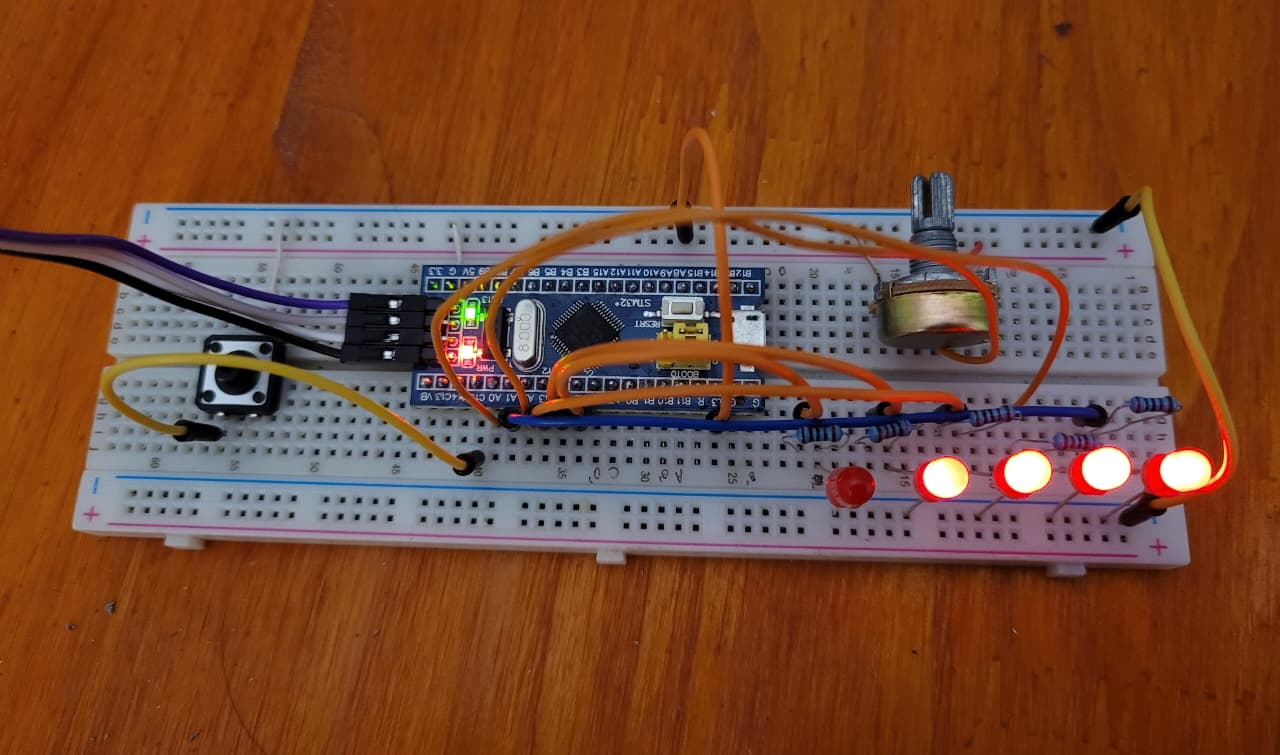
\includegraphics[width=0.6\textwidth]{images/proto.jpeg}
    \caption{Disposición del circuito en protoboard para el Ejercicio Práctico N° 2.}
    \label{fig.ej2:proto}
\end{figure}

\subsection{Inicialización y Calibración del ADC}

Para poner en marcha el ADC de forma precisa, se siguen los siguientes pasos en la función \texttt{main()}:
\begin{enumerate}
    \item Tiempos de muestreo: El sensor de temperatura interno requiere un tiempo de muestreo mínimo de
    $17.1\us$~\cite{stm32f103rm} para cargar de forma correcta la capacitancia del circuito interno de retención. Se
    escribe \texttt{0x7} en los bits 18-20 del registro \texttt{ADC\_SMPR1} para configurar el máximo tiempo de
    muestreo disponible ($239.5$ ciclos de reloj de ADC). Del mismo modo, se configura el canal 0 en \texttt{ADC\_SMPR2}
    con $239.5$ ciclos para la señal del potenciómetro externo.
    \item Activación de sensores internos y alimentación: Se escribe un '1' en el bit 23 (\texttt{TSVREFE})
    del registro \texttt{ADC\_CR2} para encender el sensor de temperatura. Se configuran los bits 17-19 de
    \texttt{ADC\_CR2} como \texttt{0b111} (\texttt{EXTSEL = SWSTART}) y el bit 20 como '1' (\texttt{EXTTRIG = 1}) para
    habilitar el inicio de la conversión por software a través del evento \texttt{SWSTART}. Posteriormente, se escribe
    un '1' en el bit 0 (\texttt{ADON}) de \texttt{ADC\_CR2} para alimentar el periférico.
    \item Calibración: Se genera un retardo por software corto para esperar la estabilización del circuito de
    conversión analógico. Luego, se escribe un '1' en el bit 2 (\texttt{CAL}) de \texttt{ADC\_CR2}. El hardware del
    STM32 ejecuta de forma automática una rutina para compensar los errores de desviación (offset) internos, y limpia
    el bit cuando el proceso finaliza. El código realiza una espera activa sobre este bit.
\end{enumerate}

\subsection{Lógica de Conversión por Muestreo (Polling)}

Dentro del bucle de ejecución principal \texttt{while(1)}, se realiza el siguiente ciclo para procesar la conversión:
\begin{enumerate}
    \item Selección de Canal: Se verifica la variable global \texttt{channel\_mode} gestionada por la ISR.
    Si su valor es 0, se escribe el valor 16 (canal de temperatura) en el registro de secuencia \texttt{ADC\_SQR3}. Si es 1,
    se escribe el valor 0 (canal externo del potenciómetro).
    \item Disparo de Conversión: Se escribe un '1' en el bit 22 (\texttt{SWSTART}) de \texttt{ADC\_CR2} para
    niciar la adquisición de la muestra.
    \item Espera de Fin de Conversión (EOC): El firmware permanece en un bucle \texttt{while} esperando que el
    hardware establezca en '1' el bit 1 del registro de estado \texttt{ADC\_SR} (\texttt{EOC}, End of Conversion).
    \item Lectura de Datos: Una vez finalizada la conversión, se lee el registro \texttt{ADC\_DT} y se aplica
    una máscara para obtener la palabra de 12 bits resultante (rango de 0 a 4095).
\end{enumerate}

\subsection{Procesamiento de Datos y Visualización}

Si el canal activo es el potenciómetro externo (valores de 0 a 4095), el valor digital se divide en cinco rangos
equitativos mediante condicionales lógicos para activar una cantidad proporcional de LEDs mediante la función
\texttt{set\_leds(count)}.

Si el canal activo es el sensor de temperatura interno, el firmware realiza el cálculo de la temperatura empleando
aritmética entera para evitar el uso de funciones de punto flotante de alto costo en microcontroladores. 
La tensión medida en milivoltios se determina como:
\begin{equation}
    V_{SENSE} = \frac{ADC_{VAL} \times 3300\mV}{4095}
    \label{eq.ej2:vsense}
\end{equation}

Posteriormente, utilizando los parámetros provistos por la hoja de datos ($V_{25} = 1.43\V$ y pendiente típica de
$4.3\mV/\Celsius$), se calcula la temperatura en décimas de grado Celsius mediante la expresión:
\begin{equation}
    T\Celsius = \frac{1430\mV - V_{SENSE}}{4.3\mV/\Celsius} + 25\Celsius
    \label{eq.ej2:temp}
\end{equation}

El valor calculado se compara para activar la barra de LEDs con una escala adaptada al rango normal de funcionamiento
de la placa de desarrollo (desde menos de $26\Celsius$ hasta más de $38\Celsius$).

\section{Relación entre Archivos de Desarrollo}
\label{sec.ej2:relacion}

La interacción del firmware se define de la siguiente manera:
\begin{enumerate}
    \item La distribución del espacio de memoria establecida en \texttt{linker.ld} ubica el vector de interrupción
    externa apuntando a la dirección física del manejador \texttt{EXTI15\_10\_}\allowbreak\texttt{IRQHandler}.
    \item Al presionar el pulsador externo en PC15, se genera un flanco descendente que dispara la interrupción. El
    procesamiento de la ISR en \texttt{main.c} alterna el valor de la variable \texttt{channel\_mode} y limpia
    la bandera de interrupción en \texttt{EXTI\_PR}.
    \item El bucle principal lee de forma continua la variable \texttt{channel\_mode} y conmuta el registro
    \texttt{ADC\_SQR3} para iniciar la conversión en el canal correspondiente.
    \item Los resultados de la conversión modifican los estados del puerto \texttt{GPIOA} a través de la función
    \texttt{set\_leds}, variando la visualización en la barra de 5 LEDs de forma asíncrona a la pulsación.
\end{enumerate}
